\documentclass[aspectratio=169]{beamer}
%% Choose aspect ratio and other standard options:
% [aspectratio=169] % 16:9 (default)
% [aspectratio=43]  % 4:3 

\usetheme[institute]{tugraz2018}
%% Choose main theme variant:
% [standard]        % standard (default)
% [institute]       % with institute's graphical acronym on the left
% [minimal]         % with reduced visuals

%% Choose your font style:
%                   % Helvetica (default for Corporate Design)
% [webfont]         % Source Sans Pro (as used on tugraz.at)
% [nofont]          % no font loaded - Computer Modern Sans

%% For more options, see README.pdf

\usepackage[utf8]{inputenc}
\usepackage[english]{babel}
%% Choose your main language:
% [ngerman]   % German
% [english]   % English


%% Add your own packages, macros, etc.
% ...


%% Enter presentation metadata
\title[Short Title]{ Hierarchical architectures for spiking \\ Winner-Take-All networks}
\author{Christoph Rieger}
\date{10.01.2025}
\institute{IML}
\instituteurl{www.iml.tugraz.at}

%% Logos
\institutelogo{beamerthemetugraz/institute/igi}  % graphical acronym for [institute] theme (left margin)
% \additionallogo{figures/logo}  % additional institute/department logo (footline; optional)
% \logobar{Supported by: ...}  % sponsors (titlepage; optional)


\begin{document}

\begin{frame}[plain]
  \maketitle
\end{frame}


\begin{frame}{Outline}
  \tableofcontents
\end{frame}


\section{Introduction}

\begin{frame}{Introduction}
  \begin{itemize}
    \item Spiking vs common NN (energy efficient, more biologically plausible)
    \item Importance of hierarchical architectures
    \item Goals of this thesis
    \begin{itemize}
      \item Simulate feedback in the visual cortex
      \item Show connection between Bayesian inference and network model
    \end{itemize}
  \end{itemize}
\end{frame}

\begin{frame}{Biological background}
  \begin{columns}[onlytextwidth]
	\begin{column}{0.5\textwidth}
      \begin{itemize}
        \item Winner-Take-All networks
        \item Modular structure of the brain
        \item Hierarchical structure of the brain
        \item Feedback mechanisms in cortical hierarchies
      \end{itemize}
	\end{column}
	\begin{column}{0.5\textwidth}
      \begin{figure}
        \includegraphics[width=0.4\linewidth]{../Latex/figures/kanizsaSquare.PNG}
      \\   \footnotesize Kanizsa square, Lee TS (2003)
      \end{figure} 
  	\end{column}
  \end{columns}
\end{frame}

\begin{frame}{Biological background}
      \begin{itemize}
        \item Probabilistic brain
        \item Synaptic plasticity
        \item Spiking neural networks
        \item Winner-Take-All networks
      \end{itemize}
\end{frame}

\begin{frame}{Theoretical background}
      \begin{itemize}
        \item Bayesian inference and its relevance to neural networks
        \item Explain model... (input image, input neurons, output neurons, prior neurons, spikes, doubleexpo kernel, membrane potential, firing rates (poisson, e hoch u - i(t)), adaptive inhibition... !!!AM BESTEN MIT DER ZEICHNUNG ERKLÄREN!
         \item Nessler said that: Every synaptic weight converges to the log of the conditional probability that the presynaptic neuron has fired just before the postsynaptic neuron, given that the postsynaptic neuron fires.... Proven later in Experiment
        \item q(k) = P(Y|X,Z) Mathematically proven  

      \end{itemize}
\end{frame}


\section{Experiments}

\begin{frame}{Methodology}
\begin{itemize}
	\item Simulation was performed in Python
	\item Simulation step size was 1 ms
	\item Pixels of input images and the prior had a noise level of 10\%
\end{itemize}
\end{frame}

\begin{frame}{Ambiguous visual stimuli 1}
  \begin{itemize}
    \item Network learned to group horizontal and vertical bars into 10 groups
    \item After training ambiguous images with 1 horizontal and 1 vertical bar were shown
    \item Network was able to focus on individual bars, due to prior neurons
  \end{itemize}
\end{frame}

\begin{frame}{Ambiguous visual stimuli 2}
        \begin{figure}
        \includegraphics[width=1\linewidth]{../Latex/figures/horvertAdaptiveInh/trainingPlotCropped.png}
      \\   \footnotesize Training plot
      \end{figure} 
\end{frame}

\begin{frame}{Ambiguous visual stimuli 3}
   \begin{columns}[onlytextwidth]
	\begin{column}{0.5\textwidth}
	        \begin{figure}
        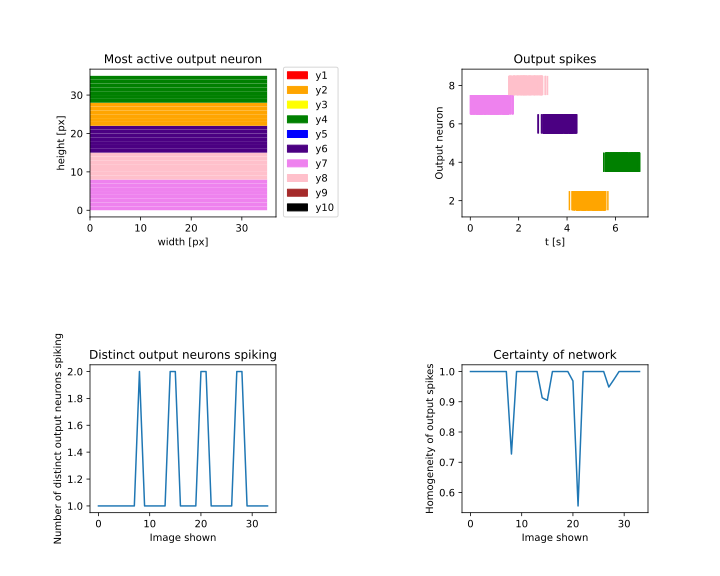
\includegraphics[width=1\linewidth]{../Latex/figures/horvertAdaptiveInh/horizontal_validation.png}
      \\   \footnotesize Horizontal validation
      \end{figure} 
	\end{column}
	\begin{column}{0.5\textwidth}
		        \begin{figure}
        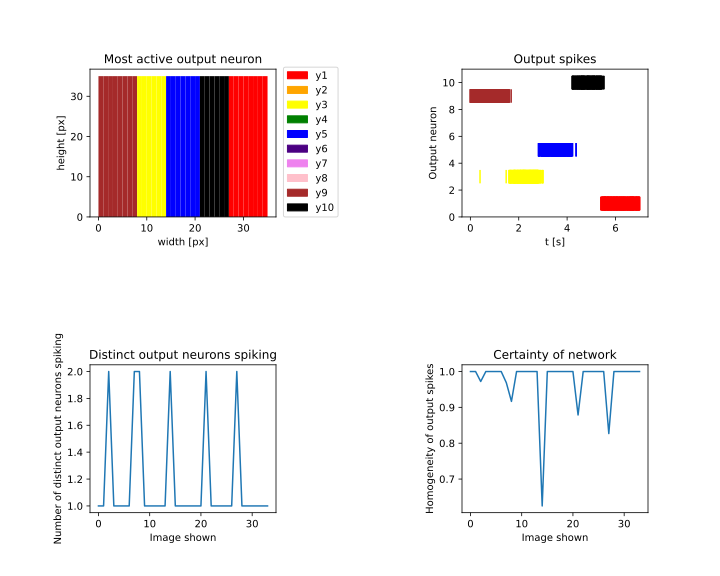
\includegraphics[width=1\linewidth]{../Latex/figures/horvertAdaptiveInh/vertical_validation.png}
      \\   \footnotesize Vertical validation
      \end{figure} 
	\end{column}
\end{frame}

\begin{frame}{Ambiguous visual stimuli 4}
 \begin{itemize}
     \item After training ambiguous images with 1 horizontal and 1 vertical bar were shown
 \end{itemize}
\end{frame}



\section{Results}



\section*{}

\begin{frame}{Conclusion}
    \begin{itemize}
    \item Biological effects could be reproduced
    \item Connection between model and Bayesian Inference was shown
    \item 
  \end{itemize}

\end{frame}

\begin{frame}{Sources}
    \begin{itemize}
    \item  Lee TS, Mumford D. (July 2003). “Hierarchical Bayesian inference in the
 visual cortex.” In: J Opt Soc Am A Opt Image Sci Vis. DOI: doi:10.1364/josaa.20.001434
    \item 
    \item 
  \end{itemize}

\end{frame}

\begin{frame}{a}
   \begin{columns}[onlytextwidth]
	\begin{column}{0.5\textwidth}
	\end{column}
	\begin{column}{0.5\textwidth}
	\end{column}
\end{frame}

\begin{frame}{a}
	\begin{itemize}
	  \item
	  \item
	\end{itemize}
\end{frame}

\end{document}
